\documentclass[letterpaper, 10 pt, conference]{ieeeconf}  % Comment this line out if you need a4paper

%\documentclass[a4paper, 10pt, conference]{ieeeconf}      % Use this line for a4 paper

\IEEEoverridecommandlockouts                              % This command is only needed if 

\overrideIEEEmargins                                     

% The following packages can be found on http:\\www.ctan.org
%\usepackage{graphics} % for pdf, bitmapped graphics files
%\usepackage{epsfig} % for postscript graphics files
%\usepackage{mathptmx} % assumes new font selection scheme installed
%\usepackage{times} % assumes new font selection scheme installed
%\usepackage{amsmath} % assumes amsmath package installed
%\usepackage{amssymb}  % assumes amsmath package installed
\usepackage{graphicx}
\usepackage{verbatim}
\usepackage{amsmath,amssymb}
\newcommand{\argmin}{\arg\!\min}
\newcommand{\argmax}{\arg\!\!\max}
\newtheorem{thm}{Hypothesis}
\linespread{0.97}
\title{\LARGE \bf
Markov Games with Time-variant Types as a Framework for Human-Robot Coordination
}
\author{Shih-Yun Lo$^{1}$, Shani Alkoby$^{2}$, Benito Fernandez$^{1}$, and Peter Stone$^{2}$% <-this % stops a space
%\thanks{*This work was supported by }% <-this % stops a space
%\thanks{$^{1}$Albert Author is with Faculty of Electrical Engineering, Mathematics and Computer Science,
%        University of Twente, 7500 AE Enschede, The Netherlands
%        {\tt\small albert.author@papercept.net}}%
%\thanks{$^{2}$Bernard D. Researcheris with the Department of Electrical Engineering, Wright State University,
%        Dayton, OH 45435, USA
%        {\tt\small b.d.researcher@ieee.org}}%
}

\begin{document}
\maketitle
\thispagestyle{empty}
\pagestyle{empty}
%%%%%%%%%%%%%%%%%%%%%%%%%%%%%%%%%%%%%%%%%%%%%%%%%%%%%%%%%%%%%%%%%%%%%%%%%%%%%%%%
\begin{abstract}
  Coordination between humans and robots commonly happens when they 
  co-exist in a shared workspace. Such scenario includes human-robot teaming on 
  collaborative tasks, and 
  human-robot conflict-resolving on limited shared resources. Mis-coordination 
  reduces 
  efficiency of both parties, and reduces the human's trust and patience with 
  the robot. In this work, we propose a game-theoretic framework to analyze 
  convergence in 
  human-robot coordination.
  We also propose human behavior hypotheses on their 
  decision-making mechanisms under this framework, 
  to capture how the human 1) perception of the robot's capabilities, 2) personal preferences, 3) level of self-interest, and 4) social 
  trust affect their policies and adaptability in dynamic environments. 
  We provide human-robot path crossing as an instantiation of our framework, and use the 
  hypothesized human behaviors to simulate real-world observed interaction 
  patterns. Lastly, we simulate humans acting adaptively to their observed robot 
  policies, as an initiative to incorporate effects on humans when designing 
  robot algorithms using human-human interaction data.
\end{abstract}
\vspace{-.2em}
\section{Introduction}
\vspace{-.2em}
Human-robot interaction has received increased attention in recent years due to the 
emerging interest in deploying robots in human environments. Such 
environments may involve human-robot collaboration on given tasks, 
humans and robots working in a shared workspace, or service 
robots deployed in human environments. In such environments, robots 
may need to coordinate with humans with partially shared information and 
partially shared objectives; agents may need to reach agreement on one 
solution among multiple feasible choices, which makes the coordination non-trivial to 
settle. For a motivating example, see Fig.~\ref{fig:intro}, which shows three agents coordinating at an 
intersection, where each agent has an individual goal to reach. 

For a robot to engage coordination without confusing the human, it first 
requires the basic capabilities to understand human intent, and to respond in a 
legible manner~\cite{dragan2013legibility}. Beyond those, to negotiate and agree on the coordinating 
solutions, the robot needs knowledge of human agents' behaviors to 
predict the outcome of its own actions. 
It also needs to known the reaction time humans need 
to update their policies~\cite{shah2011improved}, and to consider potential 
impacts of its own actions on humans' future 
decisions~\cite{fujiwara2015non,foerster2017learning}. Then the 
robot can plan and coordinate with humans in an intent-consistent fashion. 

Past research has sought to improve human-robot coordination in a variety of 
ways, including: intent-expressive robot 
motion generation~\cite{dragan2013legibility,lichtenthaler2012influence}, human 
preference-aware behavior modeling and its 
use for coordination~\cite{gombolay2015coordination,dorsa2017active}, human-robot mutual 
adaptation~\cite{nikolaidis2013human,nikolaidis2016formalizing}, human 
expectations on robot capability~\cite{cha2015perceived,kwon2016human}, as well as trust and comfort for long-term 
deployment\cite{yang2017evaluating}. 

While these topics share a focus on factors which affect human behaviors and 
their decision-making mechanisms, 
%such as reaction timing and 
%policy adaptation rate, to incorporate future impacts of robot actions into 
%robot online planning, 
they lack a unifying framework to keep track of how those factors correlate with 
each other in different situations, how they affect human 
decisions and motions, and 
how they evolve over time as a function of robot interaction policies. 
Those questions are important for designing intent-consistent robots to 
interact with humans in daily situations. And they are important for 
designing 
robots that are aware of human 
adaptation to their long-term deployments.  

   \begin{figure}[t]
      \centering
      \vspace{-1em}
      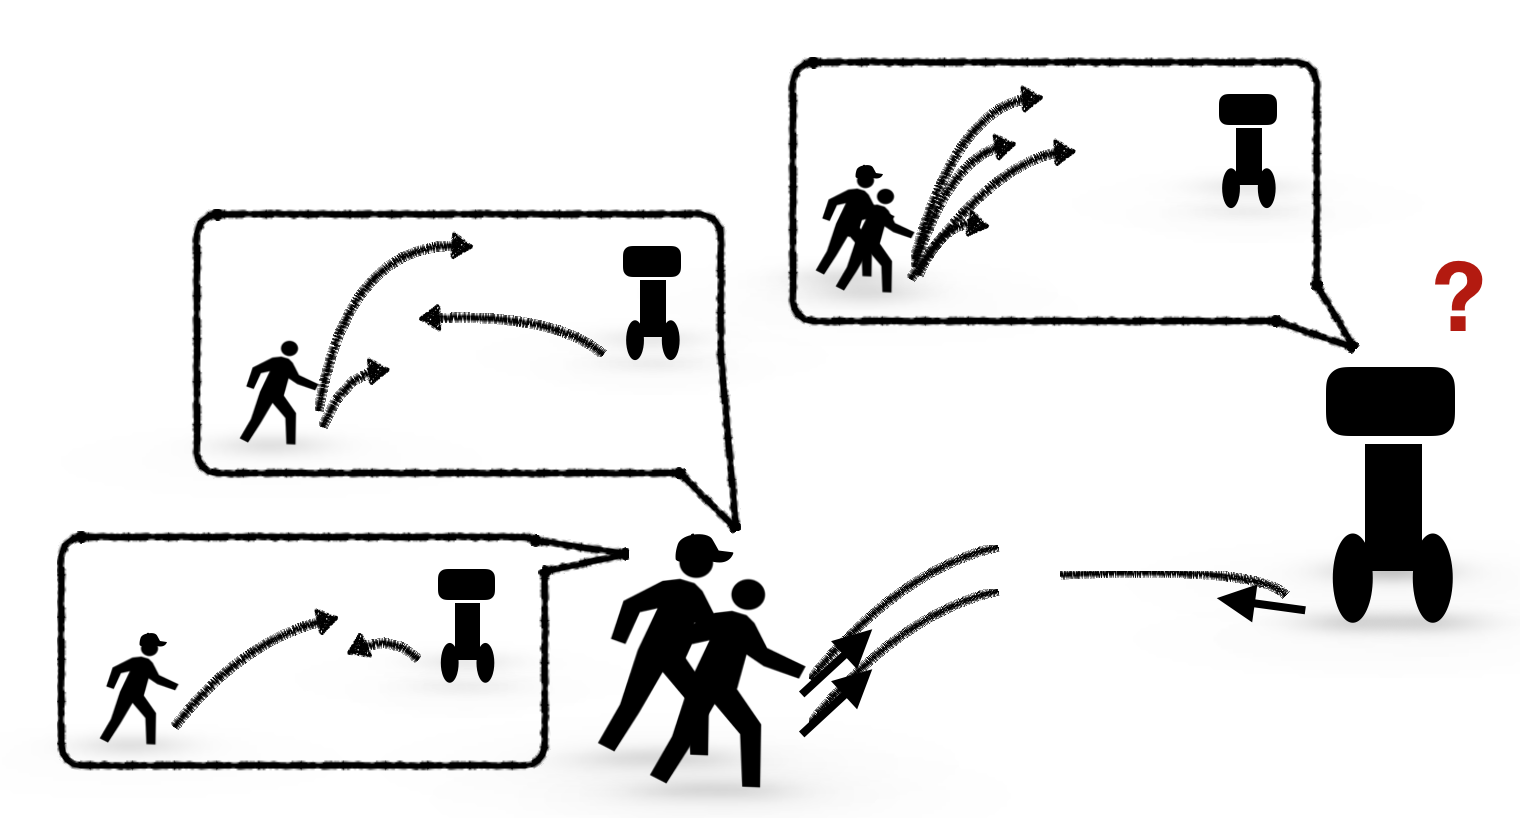
\includegraphics[scale=0.32]{intro}
      \vspace{-1.5em}
      %\hspace{-5em}
      \caption{Human-robot coordination in a crossing interaction. Since 
      people have different prior assumptions on robot behaviors, their choice 
      of actions differ.}
      \vspace{-2em}
    \label{fig:intro}
   \end{figure}
To fulfill such purposes, the main contribution of this work is a proposed game-theoretic 
model for human-robot coordination where agents have hidden preferences and time-variant adaptive behaviors based 
on online observations of others' behaviors.

To discuss human behaviors while interacting with robots, we point out some
important factors that have been proposed in the human-robot interaction 
community, such as perceived robot capability, personal preferences, and 
trust on robot ability. We illustrate how they affect human behaviors through 
our proposed human decision-making model under the game framework, using a 
receding-horizon approach. We also propose two factors that we observed to be 
important in the social navigation 
domain: level of self-interest and social trust. We incorporate them along 
with others to analyze how people interact with the robot, with different 
personal preferences and assumptions about robot 
behaviors. We collect real-world human-robot interaction data to 
illustrate our model effectiveness. 

%maybe too much, don't show..
We also use our decision-making model to discuss human adaptability to robots,
and simulate human adaptation to robots after perceiving robot 
socially trust-worthy behaviors. 

%%%%%%%%%%the algorithm: too much, don't show
%Lastly, for the robot to deploy the models to coordinate with humans 
%on-the-fly, it needs real-time 
%capabilities to update its prior knowledge 
%along interactions~\cite{sezer2015towards,bai2015intention}, 
%and then re-analyze its plan convergence criteria in coordination with other 
%human participants. We therefore propose the 
%receding-horizon planning approach, instantiate in the social 
%navigation domain. With that we show efficient robot online adaptive planning 
%to human 
%agents.   

%It is significant in highly dynamic situations, whereas good reaction 
%timing prevents 
%extra chaos or confusion. AI agents need reasoning about 
%the effect of its reaction timing, 
%the potential response to its own action, 

%We use this framework to 
%cover topics that have shown great effects on human-robot interaction, such as 
%perceived robot capability and human trust, and show simulation on how they affect 
%the coordination process on social navigation domain, in correspondence with 
%real-world observed human behaviors.  

\section{Related Work}
%motion planning: time-variant dynamics, motion legibility
%** community of planning considering human factors (existing motion planning algorithms consider: a) intent expressiveness in 
%motion generation, b) human-emulating robot navigation..)
%1. real-time fluent planning in a human-aware manner, what people have done to 
%improve from traditional planning approaches:
Despite the growing interest in deploying robots in human populated workspaces, 
motion planning algorithms for smooth human-robot coordination have remained a 
challenge. While traditional planning algorithms have shown success in static 
environments, deploying such approaches alongside humans has shown 
insufficient adaptability to highly dynamic environments, and produce awkward 
motions making 
interpretability difficult
~\cite{lichtenthaler2012influence,dragan2013legibility,kruse2012legible}. 
Approaches considering time-variant factors, such as temporal constraints for multi-agent collision 
avoidance~\cite{van2011reciprocal}, have drawn attention for such 
applications; approaches considering human factors, such as human 
collision-avoidance behavior anticipation~\cite{helbing1995social}, have also gained attention for robot planning in human workspaces~\cite{shiomi2014towards}.

On the other hand, another community solves robot planning in human environments as a 
joint multi-agent planning problem, to incorporate the collective crowd 
behaviors with explicit modeling of the effect of agent actions on its 
surround agents~\cite{trautman2010unfreezing,kuderer2012feature,mavrogiannis2016decentralized}. Such joint modeling methodology has 
shown to be effective at outputting smooth human-mimicking trajectories at the same 
time acting responsively to its surrounding agents.
%Modeling human actions 
%with explicit inputs of other agents' actions has also shown similar effects~\cite{sadigh2016planning}. 

One major drawback applying these approaches interacting with humans is that the 
multi-agent joint dynamics models are typically learnt from data collected by 
human demonstrations, whereas humans do not act the same way around a robot compared to in 
pure-human environments. This problem has shown 
inefficiency of such approaches when humans use unexpected behaviors 
around robots -- behaviors that humans will not present in front of another 
human~\cite{pfeiffer2016predicting}. 

%To keep track of the improvement in such joint modeling approach on human 
%robot interaction, we need to incorporate studies on robot factors on human 
%behavior predictive model, to plan in real-time with the right human behavior 
%prediction. we need better human model considering robots, we need a 
%multi-agent framework to describe the joint planning setting, and we need it 
%online adaptive to time-variant human behavior.  


%humans react differently around a robot, and but their knowledge and behavior 
%adapts along time during the interaction with robots. In (cite..nicklas), 
%authors address human-robot interaction considering mutual influences. In 
%(cite.dorsa), to learn from human data on how actions affect the other agents' behavior (cite..dorsa).
%planning in human environments: 
%
%To plan in response to human in a timely behavior-consistent manner: we need 
%to combine the study on robot factor on human behavior predictive model with 
%existing motion planning algorithms for robot action generation. We need a 
%unifying framework to keep track of human time-variant behavior, to respond in a way that does not introduce 


%*games in repeated form: the formulation for real-time applications is 
%unclear, fixed game outcomes 
%Markov games provide a framework for multi-agent learning  

To model joint behaviors among agents -- how one's action affects the other -- another way is to incorporate individual's action values with correlations 
with other agents' actions. Such joint behavior formulation is widely studied 
in Game theory: with different player assumptions, games evolve with different 
outcomes. In the artificial intelligence community, such game 
formulation has been incorporated with Markov Decision Process for multi-agent 
reinforcement learning~\cite{littman1994markov}. Such incorporation enables strategy 
design for multi-agent robotic systems with mutual learning. 

Yet, to simulate human-robot interaction, it requires agents modeled after 
humans, who have distinctive learning mechanisms and decision-making processes 
from reinforcement learning agents; moreover, agents have different behavioral 
types, as humans have personal preferences; agents online adapt to other 
agents, as humans observe the others and plan accordingly. Those features are 
widely studied in the human-robot interaction community, but not yet well 
formulated by one unifying framework. We therefore propose 
an extensive framework on Markov games with time-variant types to incorporate 
human-robot interaction with multi-agent learning problems to eliminate the gap. 


%\begin{table}[h]
%\caption{An Example of a Table}
%\label{table_example}
%\begin{center}
%\begin{tabular}{|c||c|}
%\hline
%One & Two\\
%\hline
%Three & Four\\
%\hline
%\end{tabular}
%\end{center}
%\end{table}


%%%%%%%%%%%%%%%%%%%%%%%%%%%%%%%%%%%%%%%%%%%%%%%%%%%%%%%%%%%%%%%%%%%%%%%%%%%%%%%%%%%%%%%%%%%%%%%%   


\section{Preliminaries}
\vspace{-.2em}
\subsection{Game Definition}
\vspace{-.2em}
Consider a game $G$ with $k$ players, where each player $i \in \{1...k\}$ has 
a finite action set $A^i$. The set of action profiles is denoted as 
$\Sigma = A^1 \times A^2 \times ... \times A^k$. The utility of an 
agent $i$ is a function, denoted as $f^i: \sigma \rightarrow \mathbb{R} $, 
evaluated at $\sigma \in \Sigma$. 

%repeated games
Games that repeat for more than one action per player are defined as 
\textit{repeated games} $G^T$, in which players receive cumulative utilities over a 
time horizon $T$, defined as:
\begin{equation}
  V^i=\Sigma_{t=0}^{T} f^i_t(\sigma_t).
\end{equation}
The action profiles $\sigma_t$ over time collectively represent the 
strategy profile $s = \sigma_0 \times \cdots \sigma_T \in S$ 

%human robot interaction as a game
We model human-robot interaction as a game, because each agent's utility not 
only depends on his or her own action, but also on others' actions. Let 
$a^H \in A^H$ and $a^R \in A^R$ be the action space of humans and robots, 
respectively. Consider a two-player game with agent $R$ and $H$, a strategy profile $s^* = (a^{R*}_{0:T},a^{H*}_{0:T})$ is a \textit{Nash Equilibrium}, if no 
agent benefits from unilateral deviation from his or her current actions:
\begin{equation}
  \forall i \in \{H,R\}, t,a^{i*}_t \in A^i, f^i(a^{i*}_t,a^{-i*}_t) \geq f^i(a^{i}_t,a^{-i*}_t). 
\end{equation}
Here $a^{-i}_t$ refers to actions at time $t$ from all agents but $i$, e.g. $a_t^{-H} = a_t^R$. 

In repeated games, agents not only need to consider the current outcome of an 
action, but also its impact on the other agents' future actions, which affect 
their own expected cumulative rewards. 

%too much.. only motivate it as games
%\subsection{Cooperative Games v.s. Non-cooperative Games}
%%too much.. not talk at all
%\subsection{Human-robot Interaction as Games}
%One common game example is social navigation~\cite{mavrogiannis2016decentralized}: each agent optimizes his or her own path to reach a final goal, while other agents' choices of trajectories may intersect and then cause delays. Agents therefore need to plan based on predictions of other agents' actions, and efficiently resolve resource conflicts.  Another example is the table carrying task~\cite{nikolaidis2016formalizing}, where agents share the same objective to collaboratively carry a large piece of furniture.
%%3. cooperative game v.s. uncooperative games
%%4. human-robot teaming v.s. co-existing in shared workspace

%Games with shared collective payoffs, $f^i=f^{-i}$, are categorized as 
%cooperative games, which are often discussed separately from those with 
%individual outcomes, especially those with profit conflicts: the 
%\textit{non-cooperative games}. For cooperative games, there is only one 
%strategy profile that maximizes the collective payoff; whereas in 
%non-cooperative games, multiple Nash equilibria may exist. In those games, 
%cooperative behaviors may also be observed based on mutual trust~\cite{fujiwara2%015non}, 
%but oftentimes self-interested strategies such as \textit{early commitments} 
%and \textit{threats} are applied to maximize personal game outcomes.

%In either, common topics such as how player \textit{trust and 
%perceived capability} affect the joint performance in human-robot interaction, 
%and how human \textit{level of self-interest and personal preferences} affect 
%the interaction, can be jointly discussed in the game framework (detailed in Sec.~\ref{sec:human_behavior}).  

%%how he or she predicts the other agents' behaviors; whereas \textit{self-interest level and personal preferences} affect his or her own utility function to parametrize game outcomes. Details will be discussed in Sec. on human behaviors and interactions with robots. 
\vspace{-.2em}
\subsection{Markov Games}
\vspace{-.2em}
Markov games~\cite{littman1994markov} are defined on top of Markov Decision Process, with finite state space 
$s \in S$, finite action space $a \in A$, and other agents' action space 
$a' \in A'$.  Agent reward 
function is a function of the state, action, as well as other agents' actions: 
$r(s,a,a')$. The framework is commonly used for multi-agent reinforcement 
learning, where agent action value $Q(x,a)$ is defined to take in the other agents' actions:
\begin{equation}
  Q(s,a,a') = r(s,a,a') + \gamma \Sigma_{s'}\mathcal{T}(s'|s,a,a')V(s'),
\end{equation}
where $\gamma$ is the discount rate, $s'$ is the state transition from 
$(s,a,a')$, $\mathcal{T}$ is the transition probability, and $V$ is the value 
function.

We propose a model, extended from Markov Games, to incorporate types as in 
Bayesian games, which assign game outcomes based on both agent actions and 
types.The model can also take in continuous-space input space $U$ to apply to real-world robotics domains. 
\section{Markov Games with Time-variant Types}
We model agents $i = 1,\cdots ,k$ to work in a joint state space $X$, where each individual has its own state 
representation $x_t^i \in X^i$ at time $t$, and control input from a bounded 
input space $u_t^i \in U^i$. $x_t = (x^1_t,\ldots,x^k_t) \in X$.

While actions $a_t^i \in A^i$ define the \textit{high-level, finite} actions an 
agent can take to affect the game outcome, $u_t^i$ defines the low-level continuous-space
realization of such options, by:
\begin{equation}\label{eq:g_function}
  u_t^i = g^i(x_t, a^i_t, \theta^i_t),
\end{equation}
where $\theta^i_t \in \Theta^i$ is some parametrization of the agent's 
(potentially) time-variant behavior.
$g^i:X \times A^i \times \Theta^i \rightarrow U$ can take in any model 
formulation, 
possibly stochastic, to sample inputs from $p(u_t^i|x_t,a^i_t,\theta_t^i)$. 
One example for high-level actions is table-turning directions; the low-level 
inputs to realize such actions are manipulator torque inputs. 
Note that, $u_t^i$ is a function of $x_t$, not solely of $x^i_t$, since agents 
adjust their motions based on other agents' status in the joint state space. 

The state transition function of agent $i$, 
$\mathcal{T}^i:X^i \times U^i \rightarrow X^i$, can then also be represented 
through
$p(x^i_{t+1}|x_t,a^i_t,\theta^i_t)$, by marginalizing over $u^i_t$:
\begin{equation}
  p(x^i_{t+1}|x_t,a^i_t,\theta^i_t) = \int_{u^i \in U^i} 
  p(x_{t+1}^i)|x^i_t,u^i_t) p(u^i_t|x^t,a^i_t,\theta^i_t)du^i.
\end{equation}

$\mathcal{T}^i:X \times A^i \times \Theta^i \rightarrow X$, as agent $i$ is 
part of the joint state; whereas the joint 
state transition function $\mathcal{T}$ takes in the form: 
$\mathcal{T}:X \times \Sigma \times \Theta \rightarrow X$, as a collective 
behavior among all agents. 

Each agent receives an immediate reward $r^i_t$ 
after taking input $u_t^i$ at state $x_t$:
\begin{equation}\label{eq:r_control_input}
  r^i_t = r(x_t,u^i_t,u^{-i}_t),
\end{equation}
where $u^{-i}_t$ is the control input of other agents at time $t$. The reward 
function $r$ considers all agents' states $x_t$ and inputs 
$u_t \in U = U^1\times \cdots \times U^k$ for evaluation.
As a result, $r: X \times U \rightarrow \mathbb{R}$; or, 
$r: X\times \Sigma \times \Theta \rightarrow \mathbb{R}$, considering the 
deterministic controller in Eq.\ref{eq:g_function}:
\begin{equation}\label{eq:r_function}
  r^i_t = r(x_t,\sigma_t,\theta_t).
\end{equation}

%\subsection{Bayesian Games with State Transitions}
%Games where agents receive outcomes depending on their own types 
%$\theta^i \in \Theta^i$ and others' $\theta^{-i} \in \Theta^{-i}$ are defined 
%as Bayesian games, where the individual 
%utility function is defined as: 
%$f^i:\Sigma \times \Theta \rightarrow \mathbb{R}$. 
%The type variable $\theta^i$ is not directly observable by other agents $-i$, 
%and an agents' policies $\pi^i$ is parametrized by his or her type, by:
%\begin{equation}
%  a_t^i \sim \pi^i(\theta^i).
%\end{equation}

%In games that involve multiple periods, an agent observe other agents' policies 
%$\pi^{-i}$, update his or her \textit{beliefs} of their types 
%$b^i_t(\theta^{-i}) \in f_{\Theta^{-i}}$, 
%and finally updates the policy $\pi^{-i}$. $f_{\Theta^{-i}}$ is some 
%probability density function over the target type space $\Theta^{-i}$. The 
%policy then takes in the time-invariant type $\theta^i$, time-variant type 
%belief $b^i_t(\theta^{-i})$:
%\begin{equation}
%  a^i_t \sim \pi^i(b^i_t(theta^{-i}))
%\end{equation}

%\subsection{Policies for Bayesian Games with State Transitions}
With the reward function $r$ defined in Eq.\ref{eq:r_function}, the optimal 
policy is then to fine the strategy $s^i$ that maximizes the cumulative 
rewards,
\begin{equation}\label{eq:optimal}
\begin{aligned}
  a^{i*}_{0:T} = \argmax_{a^i_{0:T}} 
  \Sigma_{t=0}^{T} 
  \mathbb{E}_{\theta_t,\sigma_{t},x_t|\mathcal{T},\sigma_{0:t-1}} \big{[}
  r^i(x_t,\sigma_t,&\theta_t)\big{]}+ \\ 
  V^i_{T+1}(x_T,\sigma_T,&\theta_T), 
\end{aligned}
\end{equation}
where $V^i_{T+1}$ some cost-to-go function for terminating at $\sigma_T$ at 
$t=T$.
Despite the general formalism for this framework to consider planning directly 
with the low-level control inputs $u^i_t$, discrete actions are 
computationally cheaper for plan evaluation and oftentimes easily obtained for 
domain-specific applications. Discrete action planning also well approximate 
human planning with hierarchical reasoning. 

We present the framework, as Markov games with unknown time-variant types,  
as a tool to analyze the convergence criteria of human-robot coordinating 
process. We first 
introduce general solutions for the framework in both pre-computation and 
online setting in Sec.~\ref{sec:realtime_game}; we then introduce our approximation of human 
decision-making mechanism to incorporate research topics on 
human interaction behaviors with robots in Sec.~\ref{sec:human_behavior}; 
lastly, we use the proposed model to simulate human-robot navigation with path 
crossing.

%too much..
%Consider agent 
%$i=R$, and $-i=H_1,\ldots,H_{k-1}$, for the robot to solve for the optimal 
%solution in Eq.\ref{eq:optimal}, essentially it needs knowledge of 
%how $\theta_t$ and $\sigma_t$ evolve over time. However, in real-world, only 
%$\theta^R_t$ is directly observable to the robot. Prediction of $a^H_t$ given 
%past interaction is also non-trial given unknown $\theta^{H}_t$ and their 
%occasionally irrational decisions.

%Inaccurate estimate of those parameters potentially lead to awkward 
%coordination, or even incapability to converge to a Nash Equilibrium at 
%termination.
%%we want to introduce subgame perfection NE in this work and perfect Bayesian 
%% NE, to discuss the convergence criteria given different game settings
\vspace{-.2em}
\section{Human-Robot Game in Real-time}\label{sec:realtime_game}
To formally discuss the coordinating process between humans and robots, we 
define the real-time game setting through game start and termination criteria. 
When players sense the game has started, they plan by taking other agents' 
behaviors into consideration, until they sense game termination. 
\subsubsection{Game start criteria}
%game: start
In a scenario where agents' actions affect the outcome of each other, we 
define as it meets the criterion of \textit{potential interaction}, 
$\mathcal{C}_{PI}$; when agents become aware of each other and start acting 
according to the perceived strategy of the other agents, it meets the criterion 
of \textit{mutual awareness}, $\mathcal{C}_{MA}$. Once the two criteria hold, 
the game begins. 
%(A counterexample is when agents are aware of each other but their actions do not affect each other's outcome. In such scenarios, such as pedestrians walking on different sides of a traffic intersection, no potential interaction is concerned; another example is when only partial party is aware of the other agents. In that case, merely one-way adaptation among agents happens, which we do not treat as interactions.%show graph illustration)  
\subsubsection{Game horizon and termination criteria}
%termination, finite-step
When interactions start at time $t=0$, the game repeats \textit{finitely} 
until a termination criteria 
$\beta: X \times \Sigma \rightarrow \{True,False\}$ is satisfied. It may be a 
predefined criteria, $t>T$, where $T$ is a pre-specified time frame of 
mandatory co-working. Termination criteria may also take in a dynamic format, 
such as to end the game whenever $\mathcal{C}_{PI}$ no longer holds. An 
example would be crowd interactions: when pedestrians are past the route 
intersections with one another, the game terminates; as no further intervention is 
expected.

With the above definition of game start and termination, the overall game, in 
a simultaneous-move fashion, is shown in Fig.~\ref{fig:game_tree} as an extensive-form game.
   \begin{figure}[t]
      \centering
      \vspace{-3em}
      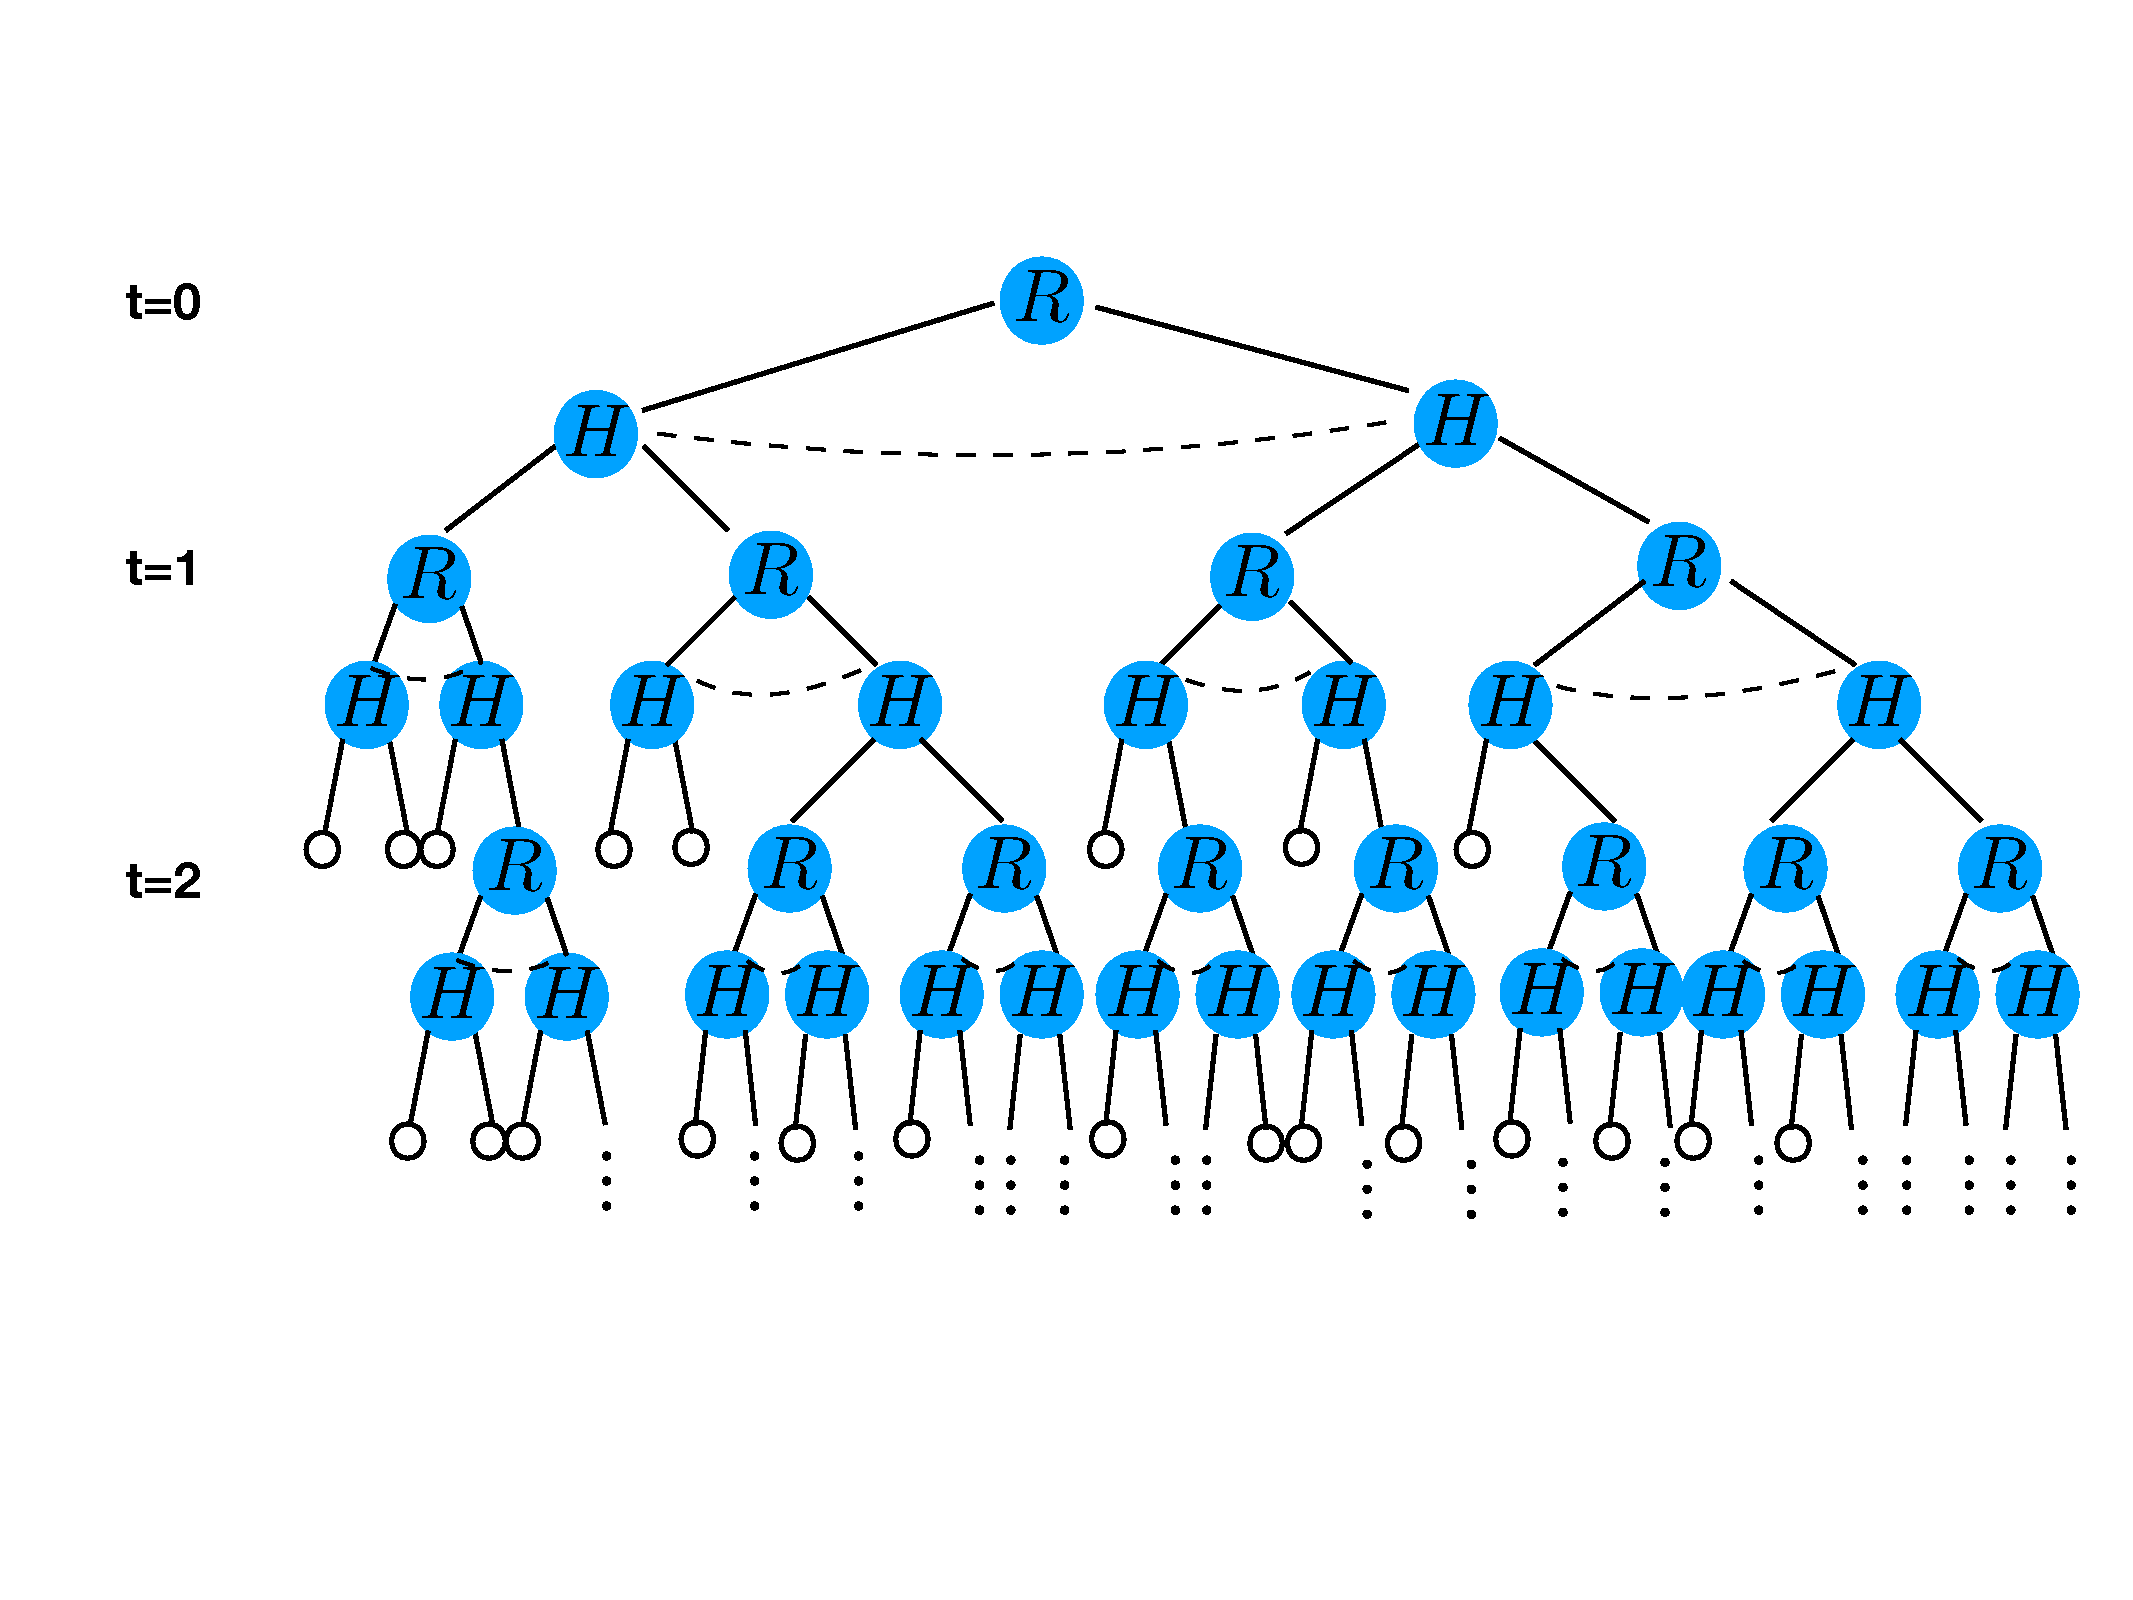
\includegraphics[scale=0.21]{game_tree}
      \vspace{-5em}
      %\hspace{-5em}
      \caption{Two-player human-robot interaction, modeled as a 
      simultaneous-move game. }
      \vspace{-1.4em}
      \label{fig:game_tree}
   \end{figure}

\vspace{-.2em}
\subsection{Simultaneous-move game tree}
\vspace{-.2em}
%basic tree introduction
The tree contains the following:
\begin{enumerate}
  \item Decision nodes: the solid circles where players make choices, 
    $a^i_t \in A^i$, based on current state $x_t$
  \item Terminal nodes: the hollow circles at the bottom where game outcomes 
    $V(x_T,\sigma_T,\theta_T)$ are assigned
  \item History set: the observed history plays before current time $I^i_t$. 
    decision nodes connected with a dashed line share the same history 
    set; players cannot distinguish nodes with the identical history sets. Therefore, in games with simultaneous moves, players share the same 
    history set in one period.  
\end{enumerate}

The policy of how an agent $i$ makes the high-level decision can be 
abbreviated as a function of his or her type $\theta^i_t$,
\begin{equation}
a^i_t \sim \pi^i(x_t,\theta^i_t|\sigma_{0:t-1}),
\end{equation}
without loss of generality.

More specifically, at each decision node, the player chooses an action based on current state $x_t$, and the policy, as to optimize Eq.~\ref{eq:optimal}, is to 
compute the following at each decision node:
\begin{enumerate}
  \item $p(\sigma_{t}|I^i_t,x_t)$: game action profile probability given history set
  \item $r_{t}$ or $V_T$: 
    reward estimate, or value estimate at termination nodes
\end{enumerate}
%$\theta^i_t$ contains three components: 
%$\theta^i_t = (\theta^i, b^i_t(\theta^{-i}_t),b^i_t(a^{-i}_t))$. 
Note that, to compute the game outcome, here we use either cumulative reward, as 
commonly seen in Markov Decision Process, or terminal value, as commonly seen 
in extensive-form games. The form of game outcome has no effect on the 
solution algorithm.  

Due to the continuous-space state space formulation, backward induction, a common 
solution for extensive-form games, is no longer applicable. Instead, 
forward-search approaches such as Monte Carlo Tree search can be applied: at 
each iteration, randomly sample an action $a^i_t$ and then expand the search 
tree by sampling the action profile 
$p(\sigma^t|I^R_t,x_t)$. To 
compute the reward of a stage game $r_t$, or the value at termination nodes $V_T$, Eq.~\ref{eq:r_control_input} can be applied by sampling $u_t$ from 
Eq.~\ref{eq:g_function}, given prior on other agents' types $p(\theta^{-i}_t)$. 
%players observe past interactions to predict other agents' 
%future policies 
%$\pi^{-i}(x_t,\theta^i_t|\sigma_{0:t-1})$, and to estimate the type parameter 
%$\theta^{-i}_t$ for game outcome estimate $\hat{V}^T(x_T,\sigma_T,\theta_t)$. When new 
%observations come in, both the predictive model on other agents' policies and 
%the type parameter estimate are updated. 
\vspace{-.2em}
\subsection{Online game strategies}
\vspace{-.2em}
When planning for long-horizon purposes, agents ideally 
want to optimize their outcome considering full-horizon accumulation, as introduced in 
Eq.~\ref{eq:optimal}. However, due to the high uncertainty in dynamic 
environments, pre-computed solutions may not fit well to newly received 
observation data, which affects agent's inference of the other 
agent: their future action profiles, their action realizations, or state transitions. Therefore, when 
playing in real-time, agents need constant online re-planning to adapt 
to unmodeled dynamic situations. 
%\begin{equation}
%    a^{i*}_{0:T} = \argmax_{a^i_{0:T}} \mathbb{E}_{a^{-i}_{0:T}} \big{[}\Sigma_{t=0}^{\beta_t=True} \gamma^t r^i(s_t)\big{]}. 
%\end{equation}

With that said, instead of running search algorithms to solve for the total 
horizon at $t=0$, agents run \textit{belief updates} whenever new 
observations arrive, and 
\textit{replan for certain horizon} from current time $t$, for as much 
lookahead horizon as computational resource allows. 
We assume agents have knowledge of the termination timing even in the dynamic setting $\beta_t$. 
\subsubsection{belief updates}\label{sec:belief_update}
During real-world interactions, observations can be from direct measures, such as 
the relative positions and velocities of all agents. Observations can also 
be implicit as to infer private messages, through ways like eye contacts or body 
languages, to express messages such as intent~\cite{knepper2017implicit}.
%While the topics of inferring human intent are non-negligible in human-robot 
%interaction (cite..), in this work, we explicitly exclude the discussion on 
%robot planning with ambiguous human expressions (cite..); we focus on 
%interactions where the action spaces of all agents are well defined and can be 
%easily understood by all parties. Details on such approximations can be seen 
%in Sec.

In either form of observations $o_{0:t}$, for long-horizon planning on 
Markov games with time-variant types, agents 
update their beliefs of the following:

(a) type estimate of other agents $b^i_t(\theta_t^{-i})$: 
$p(\theta^{-i}_t|o_{0:t})$, to sample state transitions $\mathcal{T}$ and 
compute reward function $r_t$

(b) future strategy profiles of other agents $b^i_t(\sigma_{t:T})$: 
    $p(\sigma_h|I^i_h)$, where $t\leq h\leq T$ is the future time step of interest
%on the predictive model of other agents' reactive policy:
%$z^i_t = b^i_t(\pi^{-i}(x_t,a^i_t,\theta^{-i}))$

%\subsubsection{predictions on future actions}
%The policy 
%$\pi^i:X\times \Pi^{-i} \time \Theta \rightarrow A^i_t$ computes the 
%optimal solution by the following formulation:
%\begin{equation}
%  a^{i*}_{0:T} \sim \pi^i(x_0,b^i_t(\pi^{-i}(x_0,a^i_{0:T},\theta_t),\theta_t|\mathcal{T}).
%\end{equation}
%$a^i_t \sim \pi^i(x_t, b^i_t(\pi^{-i}(x_t,a^i_t,\theta^{-i})),\theta^i)$
%\subsubsection{Termination value estimate}
Belief updates are usually computationally cheap, so agents may run it at a high 
rate (potentially higher than replan frequency) to deal with noisy 
observations. 
\subsubsection{Receding-horizon planning}\label{sec:receding}
Due to the potential demand of fast re-planning in dynamic environments, 
agents may only be computationally available to plan for finite-step lookahead $H<T$.
Therefore, at each time step $t=h$,$h<T$, agents instead try to optimize
%\begin{equation}
%  a^{i*}_{0:H} = \argmax_{a^i_{0:H}} 
%  \Sigma_{t=0}^{H} 
%  \mathbb{E}_{\theta_t,a^{-i}_{t},x_t|\mathcal{T},\sigma_{0:t-1}} \big{[}
%  r^i(x_t,\sigma_t,\theta_t)+ \hat{V}^i_{H+1}(x_H,\sigma_H,\theta_H)\big{]}, 
%\end{equation}
%\begin{equation}
%   a^{i*}_{0:H} = \argmax_{a^i_{0:H}} \mathbb{E}_{a^{-i}_{0:H}} \big{[}\Sigma_{%t=0}^{\beta_t=True} \gamma^t r^i(s_t) + \hat{V}^i_{H+1}(s_H)\big{]}, 
%\end{equation}
%where $H< T$ is a fixed horizon for lookahead, and 
%When the interaction continues, $t=h$, where $0<h<T$, 
for $t=h:H'$, where $H'=min(h+H,T)$, based on updated model of future strategy 
anticipation of other agents' $p(\sigma_{h:H'}|I^i_h)$. This online replanning 
for finite horizon strategy, known as receding-horizon planning, can be formulated as the following:
\begin{equation}
  \begin{aligned}
  a^{i*}_{h:H'} = \argmax_{a^i_{h:H'}} 
  \Sigma_{t=h}^{H'} 
  \mathbb{E}_{\theta_t,\sigma_{t},x_t|\mathcal{T},I^i_t} \big{[}
    r^i(x_t,\sigma_t,&\theta_t)\big{]}+ \\
    \hat{V}^i_{H'+1}(x_H,\sigma_H,&\theta_H), 
  \end{aligned}
  \end{equation}
where $\hat{V}_{H+1}(x_H,\sigma_H,\theta_H)$ is the cost-to-go estimate for 
following $\sigma_H$ from $t=H+1$ to $T$.

For coordination games, it is usually true that the earlier the termination, 
the better the final outcome is: similar to games with benefit discounts. Take 
the table turning task for example, the faster the two agents 
reach agreement on the direction to go, the faster progress they make, despite 
the potentially longer routes. Therefore, biased search to 
strategies with early termination has its empirically advantage; agents 
can even trade off computation depth with breadth to better explore its action profile. 

%\begin{equation}
%  a^{i*}_{h:H'} = \argmax_{a^i_{h:H'}} \mathbb{E}_{a^{-i}_{h:h+H}|s_{0:h-1}} \big{[}\Sigma_{t=h}^{H'} \gamma^t r^i(s_t) + \hat{V}^i_{H'+1}(s_H)\big{]}, 
%\end{equation}
%which is to plan for certain $H'\leq H$ horizon, execute action and observe 
%other agents' behaviors, update the belief of agents' strategies, and plan 
%again at the next time step with updated $H'$ horizon.

%\subsection{Real-time Game Formulation}
%Therefore, to analyze how human factors affect the dynamics of human-robot interaction and the game convergence over time, we propose a real-time game setting defined by the following:
%% formulation: finite time step, discount factor, start criteria, termination criteria
%\subsubsection{Game outcome and discount factor}
%value definition
%The game outcome $V^i$ of each player $i$ is defined as the discounted cumulative reward till game termination:
%\begin{equation}
%  V^i = \Sigma_{t=0}^{\beta_t=True} \gamma^t r^i(s_t),  
%\end{equation}
%where $\beta_t$ is short for $\beta(x_t,s_t)$ and $0<\gamma \leq 1$ is the discount rate.

%In the repeated game setting, the strategy profile $\mathcal{s}_{t:t+h}$ is composed by the action profiles $s_{t:t+h}$ over certain horizon $h$: $\mathcal{S} = S_0 \times S^1 \times... \times A^h$.

%\subsection{Early termination}
%A game may early terminate when a Nash Equilibrium is reached before termination and no agent conveys intent to deviate.
%---------(Recap finitely repeated game convergence, 
\section{Human Behavior and Decision-Making Model}\label{sec:human_behavior}
As one of the main purposes of our proposed framework is to model \textit{human} 
interaction with AI agents, here we introduce our hypotheses on human 
behaviors and their decision-making mechanism; by implementing these hypotheses 
into the framework, we have can better analyze how different paradigms in 
human-robot coordination affect the overall convergence.

\vspace{-.2em}
\subsection{Adaptability to other agents}\label{sec:adaptability}
\vspace{-.2em}
Humans observe other agents and adapt their strategies 
accordingly~\cite{nikolaidis2016formalizing,yang2017evaluating}. In the 
proposed framework, 
an agent's type $\theta^H_t$ is parameterized by a static parameter $z^H$, 
which is associated with his or her personal preferences that do not change in short period 
of time, and by a \textit{time-variant} parameter $b^H_t(\theta^{-H}_t)$, to 
capture the agent's dynamic \textit{beliefs} of other agents' types.
More specifically,
\begin{equation}
  \theta^H_t = \begin{bmatrix}
    z^H \\
    b^H_t(\theta^{-H}_t).
  \end{bmatrix}
\end{equation}
  $z^H$, the static type parameter, features personal 
  preferences such as travel efficiency versus travel energy in navigation 
  domains. $b^H_t(\theta^{-H}_t)$, the time-variant parameter, features 
  human's perception on other agents' types. 
  As for the detailed form in the belief, we hypothesize that 
  humans possess certain \textit{information budget} to reason about other agents' behaviors.

 Below, we propose our hypothesis on the human's information budget, which 
 corresponds to their computational capability to infer about other agents' 
 decision-making model. The decision-making model is the policy that outputs 
 the agent's high-level action(s):
 \begin{equation}
   a^i_{t:t+H} \sim \pi^i(x_t,\theta^i_t)
 \end{equation}
\subsubsection{$b^i_t(\theta^{-i}_t) = \emptyset$} 
Agents keep no information of the 
other agents' behavior; they parametrize their policies solely based on personal 
preferences, but make no use of other agents' behaviors to characterize the 
game outcome. We assume human behaviors to not belong to this 
category while interacting with robots: $b^H_t(\theta^{-R}_t)$.

\subsubsection{$b^i_t(\theta^{-i}_t) = \hat{z}^{-i}$}
Agents assume the other agents maintain no information of themselves, but only 
act according to their static preferences $\theta^{-i}_t = z^{-i}$. Therefore, 
agents adapt to the others as if their own actions have no impact on other 
agents' decision-making model: $p(a^{-i}_{t+H}|x_t, z^{-i})$. This is referred 
to as the \textit{one-layer} inference.

\subsubsection{$b^i_t(\theta^{-i}_t) = 
[\hat{z}^{-i}, 
\hat{\hat{z}}^i]$}
Agents assume the other agents are also adaptive to themselves,
$\theta^{-i}_t = [z^{-i},
\hat{z}^{i}]$, with one-layer inference. 
Therefore, when planning for more than one period, agents act adaptively, at 
the same time evaluating their actions' potential impacts on the other agents' future 
strategies. When planning for one period, Agents have the budget to compute 
two-layer inference: to plan according to what they predict the others' 
predictions about themselves 
$a^i_t \sim \pi^i(x_t, b^i_t(\pi^{-i}(x_t,b^{-i}_t(\pi^i(x_t,\hat{\theta}^i)))))$
. This is the maximum budget we assume humans can afford for real-time 
inference, and is not applied for planning due to its 
intrinsic complexity. 

Therefore, with the information budget assumption $b^H_t(\theta^H_t) = \hat{z}^{-H}$, we consider human policies 
being adaptive to their perceived, presumably static, behavior of other 
agents. The higher adaptation rate is, the more flexible they 
appear in the joint policy. 

%too much to show..
%However, due to the coupled terms on other agents' personal preferences $z^{-H}$ 
%as well as the assumed perceived preferences by other agents $\hat{z^{H}}$, 
%agents may have \textit{biased adaptation} due to \textit{biased prior} on 
%robot behavior.  
\vspace{-.3em}
\subsection{Bounded memory belief updates}
\vspace{-.2em}
As introduced in Sec.~\ref{sec:belief_update}, we also assume humans maintain their 
beliefs of other agents' types as well as their future strategy profile 
through out online planning. 
Here, we further assume humans to either run Bayesian updates, or possess \textit{bounded} memory on past observations and 
interaction history for belief updates\cite{nikolaidis2016formalizing}: $
b^H_t(\sigma_{t}|I^i_{t-(t-n)},
$
and
$
b^H_t(\theta^{-i}_t|o_{t-n:t}).
$
\vspace{-.3em}
\subsection{Finite-step lookahead}
\vspace{-.2em}
As introduced in Sec.~\ref{sec:receding}, we also assume humans to replan 
online with finite-step lookahead. 
\subsubsection{0-step lookahead, H=0}
Agents act as if the current game is the termination game. 
%If all agents plan for 0-step lookahead, players play one mixed strategy equilibrium. If there is only one equilibrium, the game converges immediately.  
%--------(proof)assuming their value estimates are consistent with the true value

\subsubsection{multi-step lookahead, H$>$0}
When agents plan as the game has more than one period, adaptive behaviors due 
to belief updates are expected~\cite{nikolaidis2016formalizing}.

%too much .. anti-adaptation
%early commitments and 
%bluffing are commonly seen to arrive at an equilibrium with higher 
%self-interests. In the real-time game setting, oftentimes one agent senses the 
%interaction and acts first, which easily allows early commitments to play the 
%role and influence other agents' strategies. Such strategies anticipate other 
%agents' strategies to be influenced by their owns: 
%$\pi^{-i}(x_0,a^i_0,\theta_0)$. 

%Such strategy is commonly seen in dense crowd navigation~\cite{knepper2017implicit}, where agents look at each other (to initialize the game through signaling awareness), act, and then quickly look away without waiting for responses. Agents then continue the same action through out the interaction and benefit from ruthless road-taking.


\vspace{-.2em}
\subsection{Anticipation of other agents' policy}
\vspace{-.2em}
%\begin{equation}
%  \pi^i(x_t,b^i(\pi^{-i}(x_t,a^i_t),\theta^{-i}),\theta^i),
%\end{equation}
As pointed out in Sec.~\ref{sec:adaptability}, humans adapt their policies 
based on their beliefs of other agents' behavior.
When planning at time $t$, agents predict about other agents' 
action profile $\sigma_{t:t+H}$ based on past interactions:
\begin{equation}~\label{eq:human_decision1}
a^H_t \sim \pi^H(x_t, b^H_t(a^{-H}_{t}|\sigma_{0:t-1})).
\end{equation}

To anticipate the other agents' actions $a^{-H}_{t}|s_{0:t}$, one may assume 
their policies are non-adaptive, $a^{-H}_t \sim \pi^{-H(x_t,z^{-H})}$, 
associated with the one-layer inference.
%one may further 
%hypothesize how the others anticipate his or her own action based on past 
%interactions, 
%\begin{equation}~\label{eq:human_decision2}
%b^H_t(a^{-H}_{t}|s_{0:t}) \sim  b^H_t(\pi^{-H} (x_t, ,b_{t}^{-H}(a^H_{t}|\sigma_{0:t-1}))),
%\end{equation}
which is of two-layer inference for planning. In this paper, we discuss human 
decisions based on only one-layer inference.
%As a result, at each decision node, human maintains belief on how other agents 
%would act according to their beliefs on his or her own policy.

%% too much.. anti adaptive behaviors
%When planning with one-layer inference to anticipate the others, as in 
%Eq.~\ref{eq:human_decision1}, humans adapt \textit{themselves} to other 
%agents' behavior. On the other hand, planning with two-layer inference 
%anticipation assumes other agents to be adaptive to themselves as well. In 
%that case, players may choose strategies that expect the others to adapt 
%to themselves. This behavior, due to the adaptability assumption of the other 
%agent, results in potentially \textit{anti-adaptive} strategies. 

%and further, they may anticipate $N^{-H}$ steps of future reactions,   
%\begin{align}~\label{eq:human_decisionN}
%b^H_t(a^{-H}_{t}|s_{0:t})& \sim  b^H_t(\pi^{-H} (x_t, ,b_{t}^{-H}(\pi^H(...,\\
%&\pi^H (x_{t},,b_{t}^{-H}(a^H_{t}|s_{0:t})))))),
%\end{align}
%\subsubsection{Bounded computation for $N$-step anticipations}
%-----------------
%\begin{equation}~\label{eq:human_decision2bounded}
%b^H_t(a^{-H}_{t}|s_{0:t}) \sim  b^H_t(\pi^{-H} (x_t, ,b_{t}^{-H}(a^H_{t}|s_{0:t}))),
%\end{equation}
\section{Explaining influential factors in human-robot interaction}
As pointed out in Sec.~\ref{sec:human_behavior}, human policies for high-level 
decisions are parametrized by $\theta^i_t$, which include that person's static 
type $z^H$ and dynamically perceived types $b^H_t(\theta^{-H}_t)$ of other 
agents. With different perceptions on the other, humans act 
differently. For example, pedestrians take over others' roads when they are in 
a hurry; however, they yield when encountering the elderly. Similar situation 
applies to human-robot interaction: people have distinctive behaviors based on 
their prior assumptions of robots, which affect their policies and their 
adaptabilities when new observations come in.
%$\theta^{-H}_t$ is assumed static or dynamic by humans, which 
%plays a role when deciding how adaptive their behaviors are to other agents. 

Here we discuss how to use the proposed model to explain phenomena in human-robot interactions. 
\vspace{-1.3em}
\subsection{Static preferences}
\vspace{-.3em}
\subsubsection{Personal preferences}
As people have different perception and long-time experience in interactions 
with the environment, they preserve distinctive characteristics in their behaviors that 
do not change in short period of time. Therefore, when planning considering joint 
actions, robots should be aware of such types to plan accordingly for agent 
comfort and overall efficiency~\cite{gombolay2015coordination}. In our 
proposed framework, personal preferences contribute to agents' policy 
realizations, transition functions, and affect the joint performances. In the 
reward function, they can be characterized as feature weighting $y^i$~\cite{dorsa2017active}:
\begin{equation}
  r^i = -y^{iT}C, 
\end{equation}
where $C$ is some vector of cost function.
\subsubsection{Level of self-interest}
When agents are deployed in public environments, the notion of public welfare 
plays in to assess policy fairness~\cite{fehr2004social}. While the public welfare is the 
self-interest in collaborative tasks, in non-cooperative games, agents have incentives to 
deviate from cooperative behaviors for personal benefits~\cite{fujiwara2015non}.  
When individuals plan in a shared workspace with personal objectives to 
achieve, resource conflicts may occur. 
While cooperative policies are the most efficient for social welfare, agents 
may gain more resource allocation when playing selfishly. 
%too much..
%It has been shown 
%that people are conditionally collaborative in such situations: they sanction 
%selfish behaviors out of fairness; further, the more benefit they gain from 
%cooperative policies, the higher they sanction on others' non-cooperative 
%behaviors. 
This notion of fairness can be characterized as weighting on all 
parties' interest $\alpha^i$:
\begin{equation}
  r^{i'} = \alpha^ir^i+ \small{\frac{1-\alpha^i}{k-1}}\sum_{-i} r^{-i}.
\end{equation}

Level of self-interest $\alpha^i$ and personal preferences $y^i$ jointly contribute to the 
static preferences $z^i$.
\vspace{-.3em}
\subsection{Perceived robot capability}~\label{sec:perceived}
\vspace{-.3em}
%When deploying robots into shared workspaces with humans, people may not have prior experience working with those agents. Intention confusion, incapability in predicting future behaviors, and mistrust are commonly described in the literature in human-robot interaction. 
The gap between true robot capability and human perceived robot capability  
has shown to deteriorate both joint and individual work efficiency in 
different task domains~\cite{dragan2015effects}. 

Here, we characterize human perceived robot capability for human-robot interaction into two categories: 1) functional capability and 2) social inference capability:

\subsubsection{Functional capability}
This includes the belief of whether the robot is able to \textit{identify 
interaction}. Before engaging interactions, agents need to ensure that 
$\mathcal{C}_{PI}$ and $\mathcal{C}_{MA}$ are met by all parties, or 
confusions may arise. Due to lack of social signaling capability, such as gazes, 
humans may be uncertain whether the robot is aware of the potential 
interactions. This may result in distantly-avoiding behaviors through out the interaction, since 
people are not sure whether to engage~\cite{dragan2015effects}.
This also includes the knowledge of robot action set $A^R$, and the confidence of 
whether the robot is able to \textit{succeed in its target actions} $a^R_t$, 
especially when complex domains are considered~\cite{chen2018planning}. 

\subsubsection{Social inference capability}
This involves whether they perceive the robot to be capable of engaging the 
game with, where implicit communication may involve to 
interact~\cite{knepper2017implicit}. This includes the ability to
\textit{identify human's intended high-level actions} based on the inference from 
past observations, and to \textit{express its own intended action} in a clear, 
context-aware, or, legible manner~\cite{dragan2013legibility}. Failing to 
present such capabilities out of human expectations deteriorates human patience 
and overall efficiency on given tasks~\cite{cha2015perceived}. 

The above two perceived capabilities are prerequisites for humans to engage in the 
coordination process with robots. In complex domains, those criteria have shown to be 
challenging~\cite{knepper2017implicit}, therefore prior experiences on 
cross-training, teaching, and learning~\cite{zhang2017plan} may be required 
to prepare for natural engagement. 
\vspace{-.2em}
\subsection{Social trust}% and reciprocity}
\vspace{-.2em}
Perceived capabilities are preliminary for human trust to interact with 
robots~\cite{yang2017evaluating}, since the knowledge of the action set of the robot enables 
human prediction of robot future actions.
When there are resource conflicts in shared workspaces, 
self-interested agents may not be socially compliant to the other agents. 
In this case, trust on social collaborativity in conflicted situations, 
captured by human's belief of robot static type $b^H_t(z^R)$, 
affects human policies through their anticipation of robot policy. While 
perceiving robots as socially 
trust-worthy agents, humans predict robots to have non-hostile behaviors and 
may cooperate at ease.   

%reciprocity may be challenged, or presumably degraded, when humans constant 
%assume compliant robot behaviors. In that situation, their belief of robot 
%reaction to human action is false placed.
\section{Problem Instantiation}
%In Sec.~\ref{sec:realtime_game}, we proposed a generalized framework to analyze 
%human-robot interaction as a game, and described the receding-horizon approach 
%to deal with uncertainties in agent type $\theta^t$.
We instantiate the framework on 2-player human-robot navigation with path 
crossing, shown in Fig.~\ref{fig:intro}.
%but do not restrict the framework from other domains 
%and applications.

\vspace{-.2em}
\subsection{Intention-aware social navigation}
\vspace{-.2em}
Great progress has been made in the past two decades in pedestrian simulations~\cite{karamouzas2009predictive,zanlungo2011social}, robot navigation with human predictive models~\cite{trautman2010unfreezing,kuderer2012feature}, and 
socially-friendly robot 
planning~\cite{mavrogiannis2016decentralized,chen2017socially}, to smoothly 
deploy robots in human workspaces. In human-robot interaction community, 
robot motion intention-expressiveness has gained attention for human 
understanding~\cite{dragan2013legibility}, and the concept of trajectory 
interpretability has been applied on robot navigation in crowded 
environments to identify goals of pedestrians~\cite{bai2015intention,unhelkar2015human}. 

   \begin{figure}[t]
      \centering
      \vspace{-1em}
      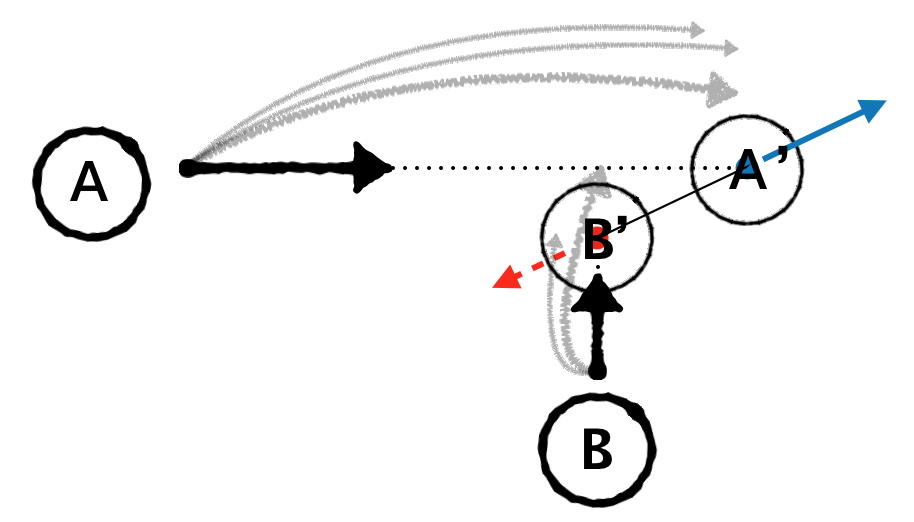
\includegraphics[scale=0.27]{pedestrian_avoidance}
      \vspace{-1em}
      %\hspace{-5em}
      \caption{Collision avoidance actions based on closest position estimate. 
      Red dashed arrow (social force direction): yielding agent with later 
      arrival timing at the intersection; blue solid arrow: passing-first agent. }
      \vspace{-1.5em}
     \label{fig:legibility}
   \end{figure}
Here we make use of the social force model with explicit collision prediction~\cite{zanlungo2011social}, which was inspired by the 
social-force model but equipped with explicit avoidance behaviors. Other 
choices of human behavioral model for action realizations 
$g(x_t,a^H_t,\theta^H_t)$ can also fit in the framework for 
simulation; we choose this model for its underlying motion \textit{legibility} 
concept in distinguishing choices of avoidance behaviors, shown in Fig.~\ref{fig:legibility}.  

When two agents have intersecting paths and have similar timing to arrive 
at the intersection, explicit avoidance behaviors are involved. Particularly, 
an agent has to decide whether to avoid in front or behind the other. This 
leaves the coordination to agree on two action combinations: (passing$\_$first,yielding), 
or (yielding,passing$\_$first).

We define the state space as the following: $x_t^R = \begin{bmatrix}
p^R_t\\
v^R_t
\end{bmatrix}$, and $x_t^H = \begin{bmatrix}
p^H_t\\
v^H_t
\end{bmatrix}$
where $p^R_t, p^H_t$ are the positions of the robot and human, and 
$v^R_t,v^H_t$ are the velocities of the robot and human, respectively. All 
variables are described in 2D, therefore, $p^R_t,p^H_t,v^R_t,v^H_t \in \mathbb{R}^2$. 
\vspace{-.2em}
\subsection{Game start and termination criteria}
\vspace{-.2em}
As pointed out in Sec.~\ref{sec:realtime_game}, to initiate interactive 
behaviors between agents, the potential-interaction criteria $\mathcal{C}_{PI}$ 
and mutual-awareness criteria $\mathcal{C}_{MA}$ are prerequisites to start the 
game. In path crossing, $\mathcal{C}_{PI}$ is met if:
\begin{enumerate}
  \item two agents have path intersections in near future: 
    $\exists t^H<t^{rH}, t^R<t^{rR}$, such that $v^R_t \times t^R + p^R_t = v^H_t \times t^H +p^H_t$
  \item the arrival timing difference is within certain threshold: $|t^H-t^R|<\delta$
\end{enumerate}
Here, the reaction time $t^{rH}$ is the timing that agents decide to 
engage in the scenario. For pedestrian avoidance, experimental results suggest 
that $t^{rH}$ is on average 4 secs before reaching the intersection~\cite{pettre2009experiment}. 
The arrival timing difference depends on agent velocities, the safety margin 
to keep from other pedestrians, and the noise in estimation. Here, we use an 
estimate value of 1.5 sec, which is the upper bound on time difference for 
which agents respond to the intersecting scenario.

The game terminates whenever two agents have passed each other, or the 
minimum relative distance has passed.

\vspace{-.2em}
\subsection{Intentions in path crossing and time delay}
\vspace{-.2em}
The action set is defined as the following: $A^R = \{a^{pf}, a^y\}$, 
$A^H = \{a^{pf},a^y\}$, where $a^{pf}$ is corresponding to the class of 
trajectory realizations to pass first, in front of the other agent; whereas 
$a^y$ is corresponding to the class to yield to the other. 

Empirical study on human-robot crossing has suggested distinctive velocity and 
trajectory profiles among two classes of avoidance 
actions~\cite{paris2007pedestrian}. Agents who intend to pass first often 
accelerate and bend their trajectories away from the other; agents who intend 
to yield often slow down. Such changes in motion profiles are clear 
signals for agent passing intents, and one can observe responses within short period of time, around 0.7 sec.



%However, due to the 
%gap between human-robot and human-human interaction behaviors, when deploying 
%robots using learnt algorithms from human crowd data, 
%state-of-the-art motion planning approaches have shown 
%large bias in human predictions~\cite{}

%Social navigation has its intrinsic complexity due to the following reasons: 
%\begin{enumerate}
%  \item agents have distinctive choices over path homotopy classes, which 
%    are associated with diverse motions
%  \item agents have personal preferences in navigation patterns
%  \item agents have adaptive navigation patterns to that of the other agents'
%  \item while the choice of homotopy classes are assigned by agent arrival timings, 
%    humans often break such assignments through changes in navigation 
%    patterns and social signaling, and expect the other agents to adapt accordingly
%  \item people choose different policies to interact with the others based on 
%    the perceived relative capability and identity. For example, adults yield 
%    more to elderlies 
%\end{enumerate}

%As a result, social navigation suffers much on prediction errors due to the 
%distinctive avoidance behaviors, and it inherits social hierarchy that is not 
%directly observable. Different human-robot interaction patterns are caused by 
%different behaviors.   

%Still, there remains the gap to bridge to take into account the 
%behavior differences when humans are around a robot and around a human. More 
%importantly, we need a robust way to model how humans adapt their behaviors 
%overtime when social robots are deployed in their environments (cite.), so we 
%can design agents that foster human adaptations of desire. 

%In real-world settings, however, agents take time to perceive intent and then reason 
%about their future actions. While the simultaneous-move setting captures the 
%nature of human-robot interaction, uncoordinated timings of decision may 
%introduce oscillations in the process. Along with the time delay  


%With proper waiting time after the initial action, the decision timing of both agents can be clearly 
%separated to prevent oscillation, which results in a form  

%, which involves 
%decisions involving longer time duration and game early termination.
   \begin{figure}[t]
      \centering
      \vspace{-1em}
      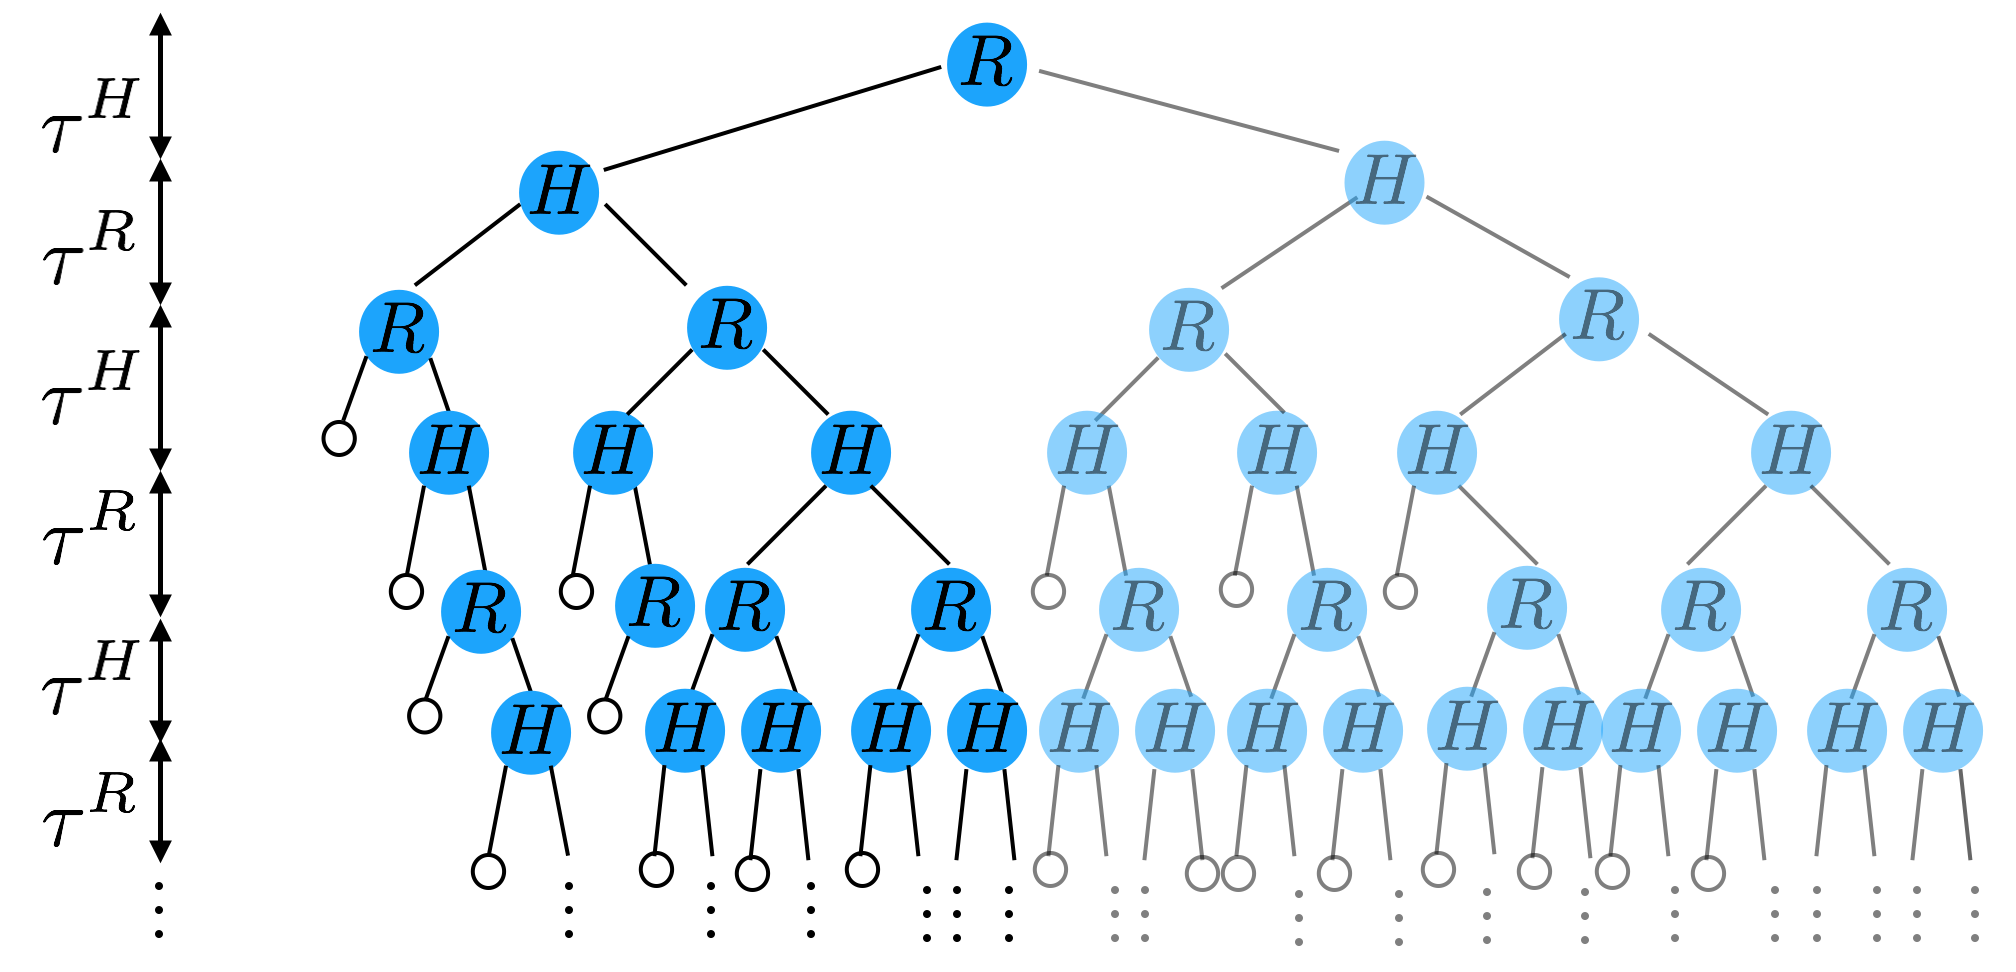
\includegraphics[scale=0.2]{turn_taking}
      \vspace{-1.4em}
      %\hspace{-5em}
      \caption{
        Human-robot turn-taking games with robot anticipating action value 
        based on finite-horizon predictions. $\tau^R$ and $\tau^H$ 
  are approximate time intervals for robot and human response times. The game may 
     terminate at either player's decision nodes.}
      \vspace{-1.5em}
     \label{fig:turn_taking}
   \end{figure}
%Despite the intention-expressive avoidance behaviors observed among 
%pedestrians, people require more than 0.5 sec to respond to perceived 
%intentions. This psychological tension in action realization, combined with 
%the decision-making process time and intent signal process time, contribute to 
%an overall reaction time
The minimum time for human agents to 
react to their action changes, $\tau^H$,
is here assumed to be between 0.7s to 0.9s. For more complex domains, higher 
values should be considered.
\vspace{-.2em}
\subsection{Response-time-adapted turn-taking structure}
\vspace{-.2em}
While the interaction process is modeled as a simultaneous-move game in 
Sec.~\ref{sec:realtime_game}, with the time delays in action realization, it 
is often played as a \textit{turn-taking} game. With proper waiting time after 
the initial action, the decision timing of both agents can be clearly 
separated to prevent oscillations. Despite the nature in the simultaneous-move 
setting for interactions, turn-taking games simplify the simulation setting 
and therefore save computation. The overall turn-taking game used in this 
instantiation is illustrated in Fig.~\ref{fig:turn_taking}.

   \begin{figure*}[t]
      \vspace{-1em}
      \centering
      \hspace{-5em}
      \vspace{-1em}
      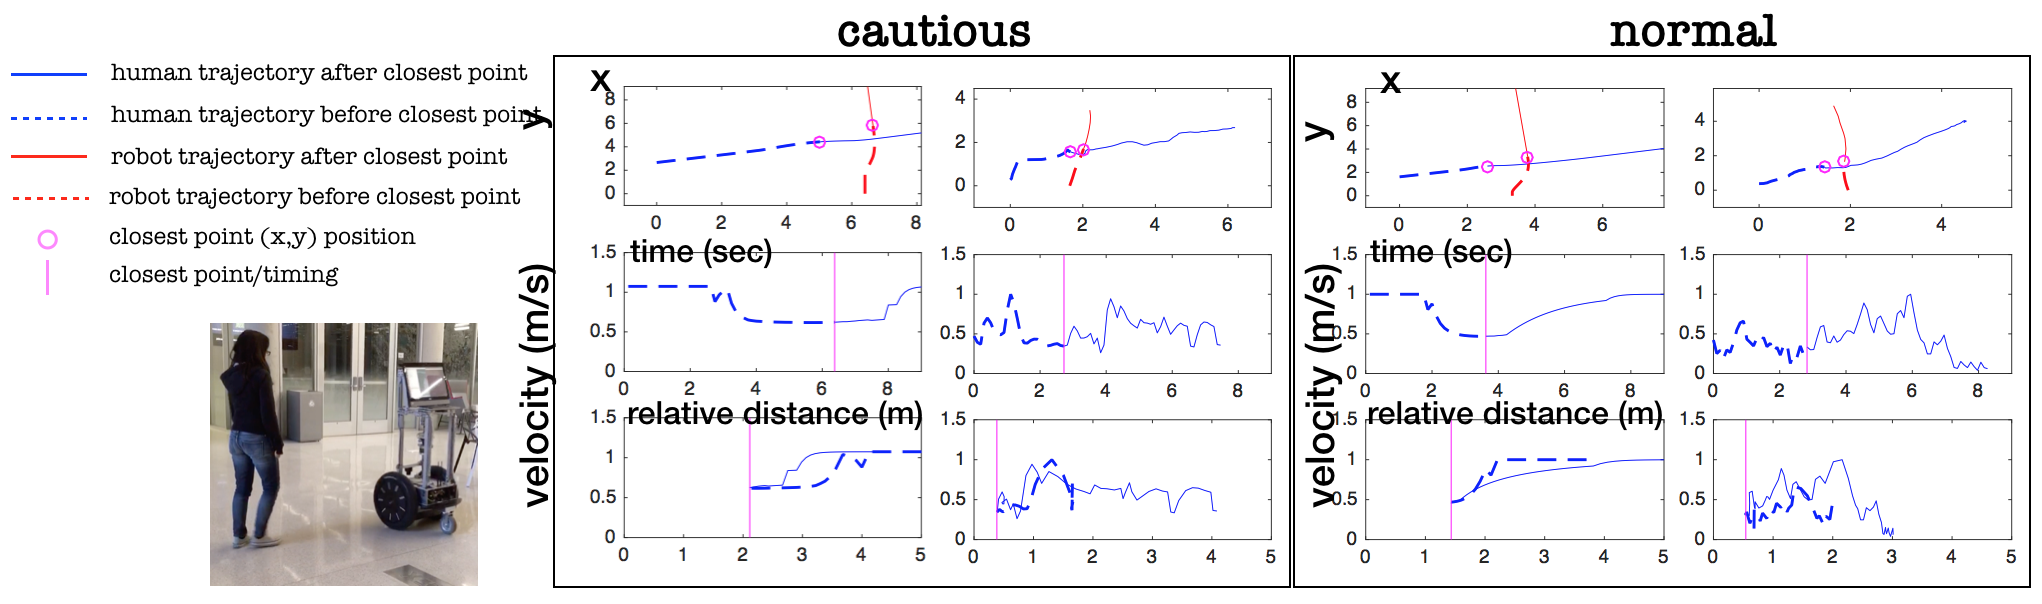
\includegraphics[scale=0.48]{iros_exp}
      \hspace{-5em}
      \caption{SIMULATED pedestrian yielding, compared with REAL recording. 
      We observed many types of behaviors during the experiments, and 
      illustrate one common type in human-robot crossing: cautious, shown in 
      the left box. Compared with people with 
      gradual slow-down and speed-up (noted as ``normal'', shown in the right 
      box), cautious agents 
      wait for the robot until it passes the intersection (shown in the 
      bottom-left photo). We simulate agent yielding and compare the x-y 
      trajectory (top) and velocity profile over time (middle) and relative 
      distance (bottom) with the true recordings, right-side of each box.   
      %While cautious 
      %behaviors may be caused by incomplete perceived robot capability as well 
      %as low belief on robot social trust, agent's attention level to the 
      %robot can differ in the two situations: we observed some agents 
      %not paying attention to the robot and walking fast past whenever 
      %nearby, which we refer to as non-engaging behavior.
      }
      \vspace{-1.5em}
     \label{fig:cautious_recording}
   \end{figure*}
%%When agents change decisions in their high-level actions $a^i_t$, the 
%low-level realization takes 
%time $\tau$ to respond: $u^i_t = g^i(x_t,a^i_{t-\tau},\theta^i_t)$. Those 
%decisions may also take time to compute.
%Further, intentions take time to convey as well as for the other 
%agents to comprehend, as the inference model 
%$p(a^i_t|x_{t-\delta:t},u_{t-\delta:t})$ 
%may not be efficient given complex domains. Therefore, in real-world 
%interaction, agents need to reason with expected response delay by other 
%agents, and to adapt to other agents in a delay-aware manner, or oscillations 
%may occur. 

%Due to the non-trial delay in response time, there are potential scenarios 
%where agents have no enough time to respond to the other agents strategies 
%before termination. We refer this as 0.5-step  
%termination. In this case, 0-step lookahead is anticipated, as no 
%adjustments from other agents can be expected.
%% extensive-form turn-taking tree introduction

%When the robot plans in the turn-taking setting, it needs to take human 
%response time into consideration to estimate game termination. As a result, in 
%situations where one of the agents may be facing 0.5-step termination, early 
%termination should be planned, as to enforce convergence for safety concerns.
\vspace{-.4em}
\subsection{Experiments}
\vspace{-.2em}
We hypothesize that our proposed framework can explain different types of 
avoidance behaviors when their paths intersect with robots. We use our 
framework to simulate a particular type, cautious behavior, in comparison with 
collected trajectory data, to show that the framework can capture distinctive 
interaction patterns among people.

We deploy a mobile robot into a building atrium, and record human crossing 
trajectories using tracking packages on laser scans~\cite{leigh2015person}. 
Eight participants were requested to head towards a set of goals, while the 
robot followed a given route that intersected with human eight times.
The robot was implemented with a 
local planner with emergent slow-down when sensing an object within 1 meter. 

With the same prior on robot strategy profile, with 0-step lookahead, 
virtual pedestrians act compliantly after observing the other agent's action, 
due to the assumption of immediate termination. With 1-step lookahead, agents assume 
the game may end with the robot playing minimax strategy, therefore they play 
based on conservative value estimate. With 2-step lookahead, virtual 
pedestrians are capable of planning for the optimistic (2nd step) in the 
worst case robot strategy (1st step). Therefore the behavior is less 
conservative compared to the previous two options. 
%While different priors give 
%different behaviors, on average, with 2-step lookahead, virtual pedestrians 
%become to yield when the estimated advance in arrival time is 0.0 sec; with 1-step lookahead, 
%agents yield when the advance becomes less than 0.6 sec. Agents with 0-step 
%lookahead act only after the other agent has acted, and their actions are 
%always compliant.  

   \begin{figure}[t]
      \centering
      \hspace{-5em}
      \vspace{-1.3em}
      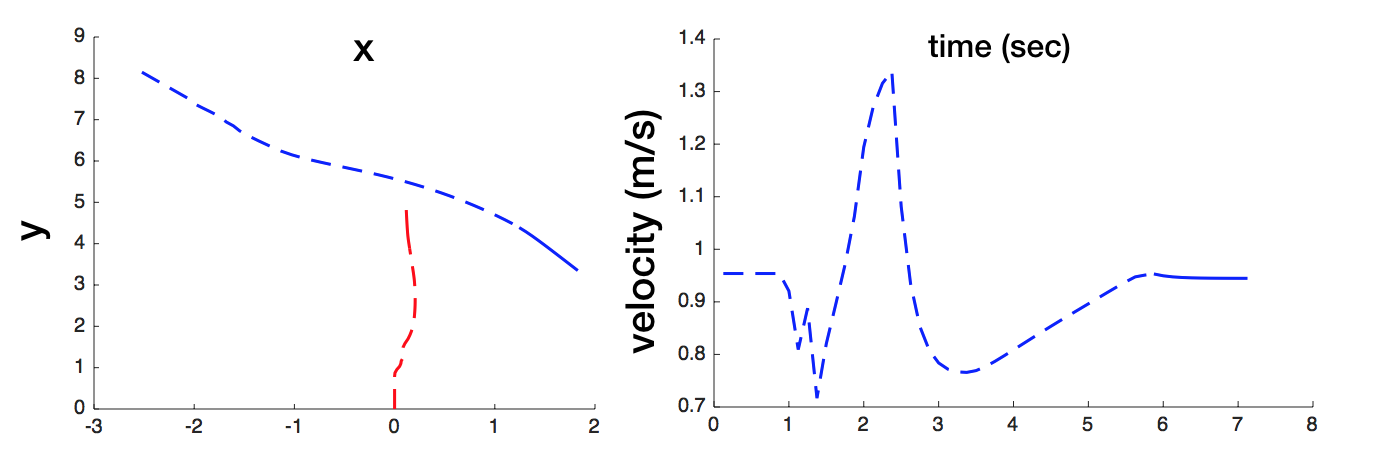
\includegraphics[scale=0.33]{adaptation}
      \hspace{-5em}
      \caption{SIMULATED cautious agent updating belief on robot strategies. While the simulated pedestrian yields at the 
      beginning (with -0.7 sec arrival timing difference), after observing 
      robot yielding behavior, she updates her 
      belief and changes the action in the next time frame.}
      \vspace{-2em}
     \label{fig:adaptation}
   \end{figure}
We simulate virtual pedestrians with type $\theta^H_t = [z^H, b^H_t(z^R)]$, 2-step 
lookahead, memory bound on interaction history = 2,  
in the turn-taking formulation. This is associated with the decision-making 
capacity to reason: ``what would the robot do after seeing my action, and what 
I could do to in reaction to that action?''. Other combinations can be 
considered. 
%High-level actions $a^H_t$ are realized 
%through the social force model with choice of collision avoidance action.
We have the robot 
%planning using the social force model with explicit collision 
%prediction, which enables the robot to decide
choose avoidance actions purely based on arrival timing estimates. It is a  simple model for demonstration clarify on human 
responses; more complex models can be used.

%preference: velocity deviation (aggressiveness v.s. social friendliness)
%self-interest: (self-interested weight v.s. social welfare)
%perceived capability: (to show largely avoidant behavior)
%trust: 
%1.(to show interactive, but frequently yielding behavior)
%2.(to show interactive, exploration behavior, probing behavior)
\subsubsection{Perceived capabilities}
Complete set of perceived capabilities are specified in Sec.~\ref{sec:perceived} as 
prerequisites for humans to engage in the coordination process with robots. 
For social navigation, when people see a robot coming, they may be unsure 
whether 1) the robot sees them (of $\mathcal{C}_{MA}$), 2) the robot is aware of the potential 
collision (of $\mathcal{C}_{PI}$), 3) when they choose an avoidance action, the robot can identify the underlying 
intention (of social inference capability on perception), and 4) when the robot 
avoid, humans can identify the underlying intention (of social inference 
capability on motion generation). 

%Since the participants mostly had no prior experience interacting with the 
%robot, we observed many non-engaging behaviors through out the passing 
%process. Two example recordings are shown in Fig~\ref{fig:cautious_recording}. 
\subsubsection{Types in path crossing}
Agents perceived other agents' behaviors and update their own type $\theta^H_t$. In 
social navigation, personal spacing is a common example, as people act 
repellently more to unfamiliar agents. People's urgency to travel to their own 
goals are common factors to describe navigation preferences. In simulation, we 
simulate agents to choose avoidance actions based on the following cost formulation:
\begin{equation}
  r^H_t = -\eta \alpha C^H_t  -(1-\alpha) C^{-H}_t,
\end{equation}
where $C^H_t$ is the estimated time delay, $\eta \in [0,1]$ is the urgency 
level, and $\alpha \in [0,1]$ is the level of self-interest.
\subsubsection{Social trust}
When navigation around a robot, the assumption of whether it is socially 
compliant affects human's avoidance decision. We commonly observe, at the 
beginning of the experiment, participants slow down to wait for the robot to 
pass first, even when the robot has a later arrival 
timing; people speed up and stay far from the robot when trying to pass in 
front, even when the robot is still far from the intersection. 
We refer to this type of behavior as cautious, simulated in 
Fig.~\ref{fig:cautious_recording} through 
varying the perceived robot level of 
self-interest: $b^H_t(z^R)$. 
%With high belief on the robot's level of 
%self-interest, virtual pedestrians have higher probability to yield to the 
%robot and stay far. 
\subsubsection{Human exploration and adaptation}
We observed many conservative decisions on human crossing, where 
pedestrians constantly yield to the robot. 
There was one agent who tried to pass in front of the 
robot after a couple of times of crossing and then decided to pass first. We 
refer this process as the agent was gradually gaining social trust on the 
robot; she updated her belief of robot behavior and then adapted her own 
strategy. Similar behavior was simulated on virtual human with high belief 
update rate, shown in Fig~\ref{fig:adaptation}.   
\section{Conclusion and Future Work}
We propose a Markov Game model with time-variant types to analyze human-robot 
coordination outcome, and propose a human decision-making model to describe 
phenomena in human-robot interactions. With the framework, we simulate virtual 
pedestrians with cautious type behaviors on human-robot crossing and compare 
the results with real-world recording. We also simulate adaptive human 
behaviors through belief updates on robot policy. In future work, we will 
further investigate human adaptability criteria based on different prior 
assumptions on robot behaviors and game convergence given false human 
assumptions.
%and how we can design robot policy to trigger adaptations that 
%correct false human assumptions on robots.     
%%%%%%%%%%%%%%%%%%%%%%%%%%%%%%%%%%%%%%%%%%%%%%%%%%%%%%%%%%%%%%%%%%%%%%%%%%%%%%%%
\bibliographystyle{plain}
\bibliography{reference}
\end{document}
